%! Author = itgramic
%! Date = 05.12.23

% Preamble
\begin{flushleft}
    \subsubsection{yugabyteDB - Distributed SQL 101}
    yugabyteDB - Distributed SQL 101 ist eine nahezu komplett \Gls{PostgreSQL} Kompatible Datenbank.
    Sie ist eine Distributed SQL Datenbank, also eine Verteilte Datenbank\cite{ZXD6D9KU}.
\end{flushleft}
\begin{flushleft}
    \paragraph{Core-Features}
    Die wichtigsten Features von YugabyteDB sind\cite{N6QKEPAC}:
    \begin{itemize}
        \item PostgreSQL Kombatibel
        \item \Gls{Cassandra}-Kompatibilität
        \item Horizontal skalierbarkeit
        \item Global verteilbar
        \item Cloud Native
    \end{itemize}
\end{flushleft}
\begin{flushleft}
    \paragraph{Replikation}
\end{flushleft}
\begin{flushleft}
    \paragraph{Proxy}
    YugabyteSQL nutzt Kubernetes und seine Core-Functions als Load Balancer.\\
    Ein zusätzlicher Proxy wird nicht benötigt.
\end{flushleft}
\begin{flushleft}
    \paragraph{Pooling}
    YugabyteDB hat ein Connection Pooling mit dem YSQL Connection Manager integriert\cite{2FQ8JXD7}.
\end{flushleft}
\begin{flushleft}
    \paragraph{API / Skripte}
    YugabyteDB bietet eigene APIs\cite{ZXXLVVYW} und CLIs\cite{8846IPNK} für das Verwalten an.
\end{flushleft}
\begin{flushleft}
    Diese bieten auch die möglichkeit, abgesichert zu werden.
\end{flushleft}
\begin{flushleft}
    \paragraph{Architektur}
    yugabyteDB ist kein reines \Gls{RDBMS}, resp. gar keines.
    Die Basis besteht aus einem \Gls{Key-Value-Store}.
    Darüber wurde eine \Gls{Cassandra}-like Query API und eine PostgreSQL like SQL API aufgebaut:
    \begin{figure}[H]
        \centering
        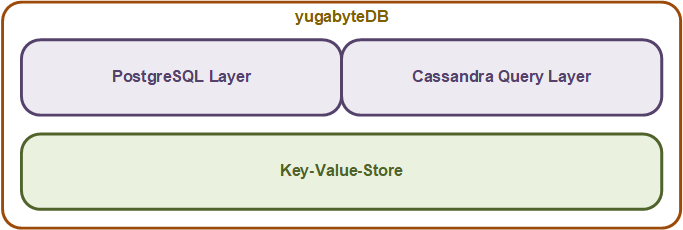
\includegraphics[width=0.8\linewidth]{source/implementation/evaluation/postgresql_ha_solutions/yugabytedb/yugabytedb-concept}
        \caption{yugabyteDB - Grundkonzept}
        \label{fig:yugabytedb-concept}
    \end{figure}
\end{flushleft}
\begin{flushleft}
    Der Basisaufbau wiederum beinhaltet diverse Dienste für das Sharding, die Replikation und Transaktionen:
    \begin{figure}[H]
        \centering
        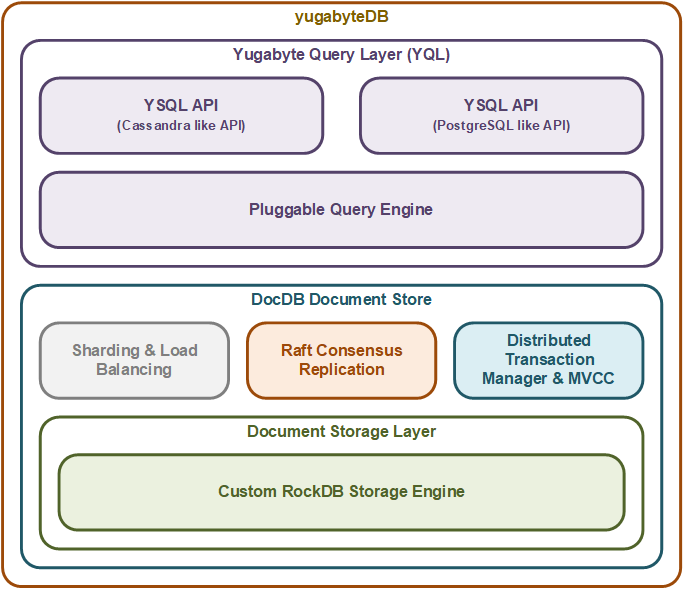
\includegraphics[width=0.8\linewidth]{source/implementation/evaluation/postgresql_ha_solutions/yugabytedb/yugabytedb-basic-archicture}
        \caption{yugabyteDB - Architektur}
        \label{fig:yugabytedb-basic-archicture}
    \end{figure}
\end{flushleft}
\begin{flushleft}
    \subparagraph{yugabyteDB - Sharding}
    yugabyteDB teilt seine Tabellen in Tablets auf.
    Die Aufteilung kann gemäss Sharding-Standards gemacht werden:
    \begin{figure}[H]
        \centering
        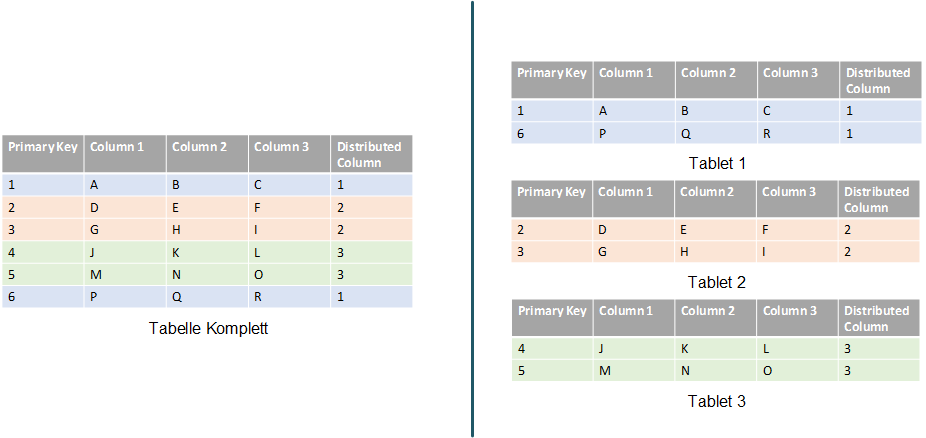
\includegraphics[width=0.8\linewidth]{source/implementation/evaluation/postgresql_ha_solutions/yugabytedb/yugabytedb-sharding-tablets}
        \caption{yugabyteDB - Sharding}
        \label{fig:yugabytedb-sharding-tablets}
    \end{figure}
\end{flushleft}
\begin{flushleft}
    Dabei hat jedes Tablet auf einem Node einen Leader, der an die Follower auf den anderen Nodes repliziert:
    \begin{figure}[H]
        \centering
        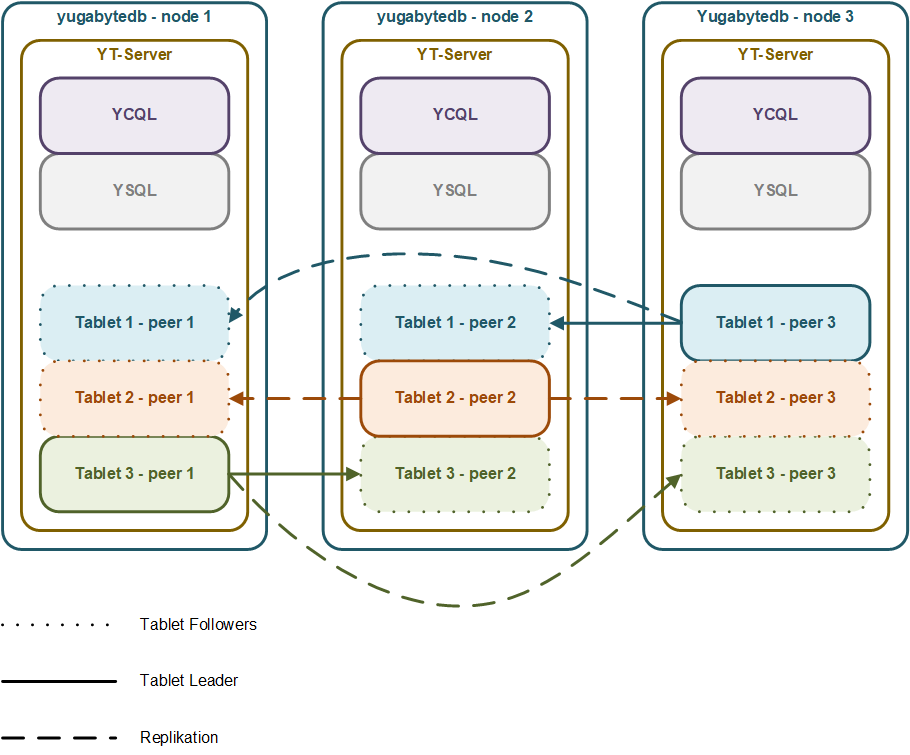
\includegraphics[width=0.8\linewidth]{source/implementation/evaluation/postgresql_ha_solutions/yugabytedb/yugabytedb-tablet-masters}
        \caption{yugabyteDB - Tablet - Leader und Follower}
        \label{fig:yugabytedb-tablet-masters}
    \end{figure}
\end{flushleft}
\begin{flushleft}
    Mit dem Replikationsfaktor  kann angegeben werden, auf wie vielen Nodes ein Tablet repliziert werden soll.
    Bei einem 4-Node System können z.B. einige Tablets einen Faktor 3 haben, dass heisst, dass die Daten nur auf 3 Nodes repliziert werden.
    Bei einem Replikationsfaktor 4 werden die Daten auf alle Nodes repliziert.
    Dies wird mit einem eigenen Service, dem YB-TServer service \cite{RSV64WED} geregelt:
    \begin{figure}[H]
        \centering
        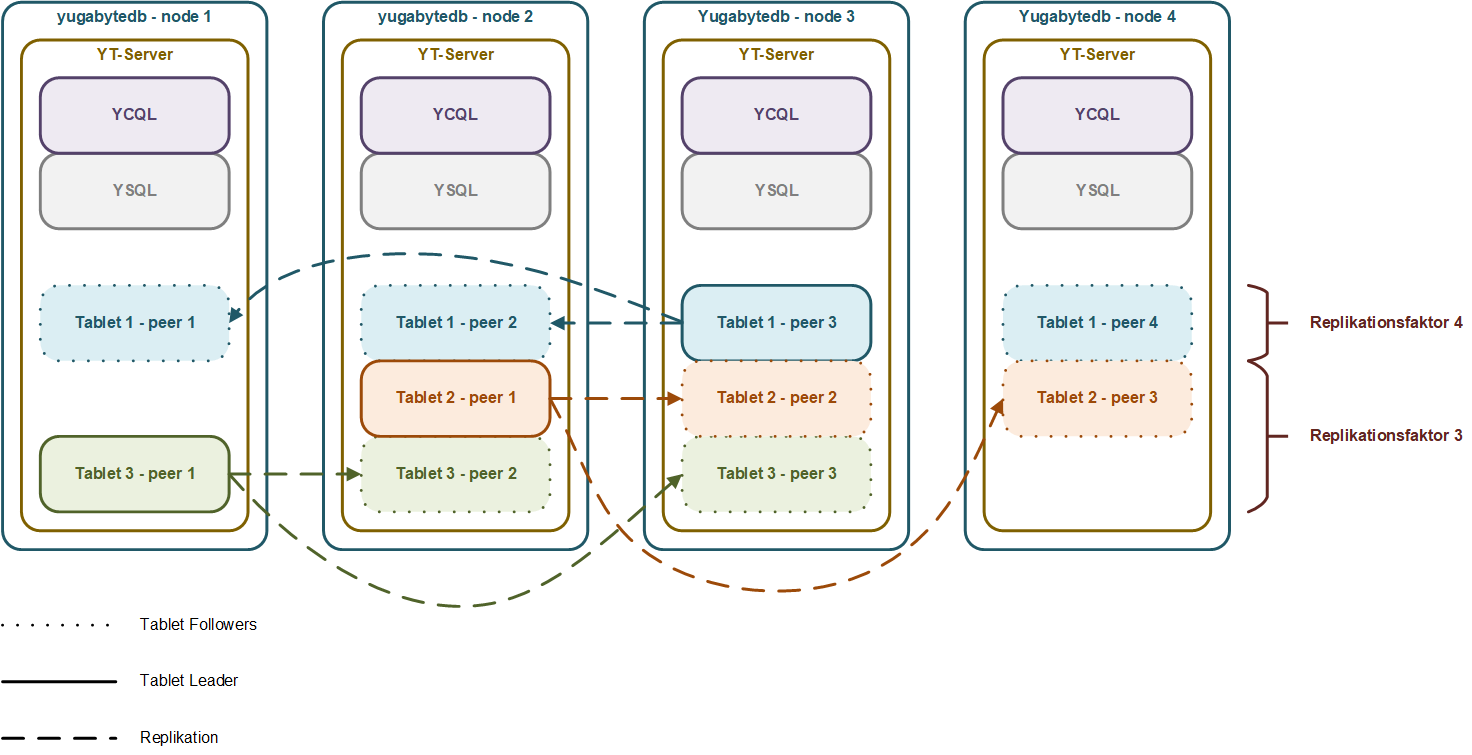
\includegraphics[width=0.8\linewidth]{source/implementation/evaluation/postgresql_ha_solutions/yugabytedb/yugabytedb-tablet-replication-factor}
        \caption{yugabyteDB - Tablet - Replikationsfaktor}
        \label{fig:yugabytedb-tablet-replication-factor}
    \end{figure}
\end{flushleft}
\begin{flushleft}
    Durch das Raft-Protokoll werden die Tablet-Leader regelmässig gewechselt.
    \end{flushleft}
\begin{flushleft}
    Mehrere Nodes können zu Zonen zusammengebunden werden, die dann z.B. auf verschiedene Rechenzentren verteilt werden:
    \begin{figure}[H]
        \centering
        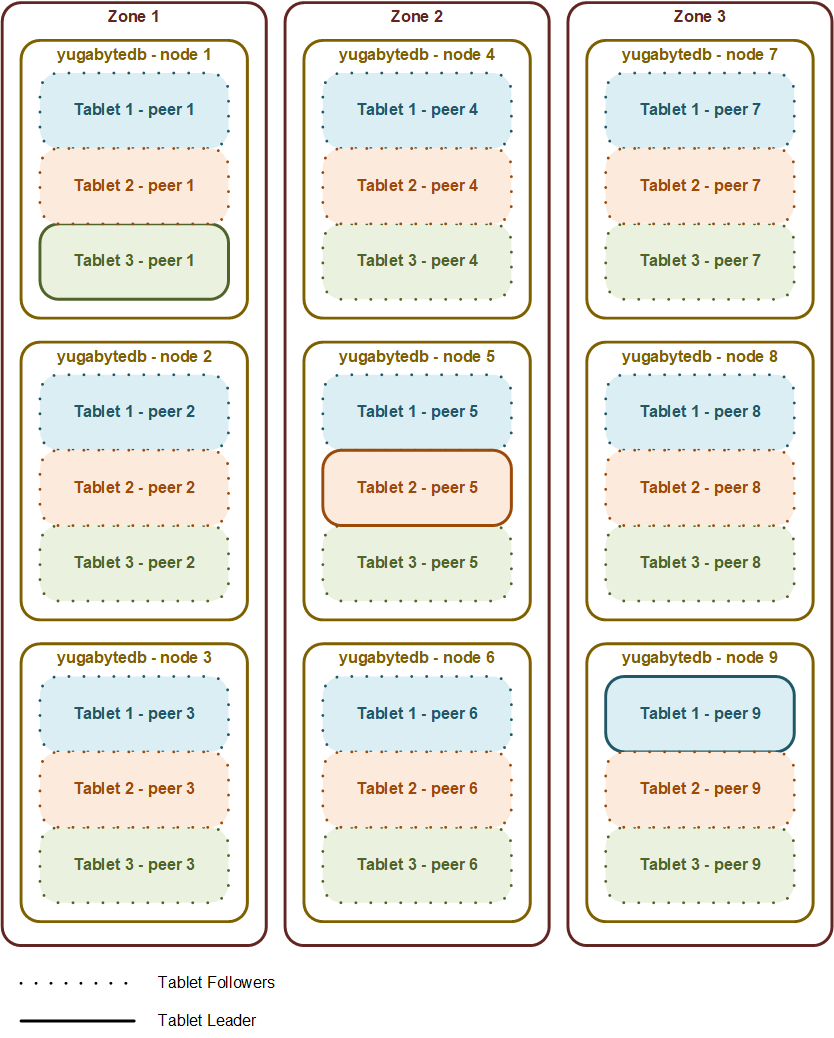
\includegraphics[width=0.8\linewidth]{source/implementation/evaluation/postgresql_ha_solutions/yugabytedb/yugabytedb-zones}
        \caption{yugabyteDB - Zonen}
        \label{fig:yugabytedb-zones}
    \end{figure}
\end{flushleft}
\begin{flushleft}
    Dies wird dann sinnvoll, wenn eine gewisse Ausfalltoleranz erreicht werden soll.
    Fällt nämlich ein Tablet Peer oder ein Node in einer Zone aus, so wird die ganze Zone sofort als nicht mehr Arbeitsfähig angesehen.
    Entsprechend werden in allen Nodes die Tablet-Leader stillgelegt und auf die übrigen Zonen verteilt.
    YuganyteDB nennt dies \texttt{Zone outage Tolerance}\cite{PTKCP8A4}.
    \begin{figure}[H]
        \centering
        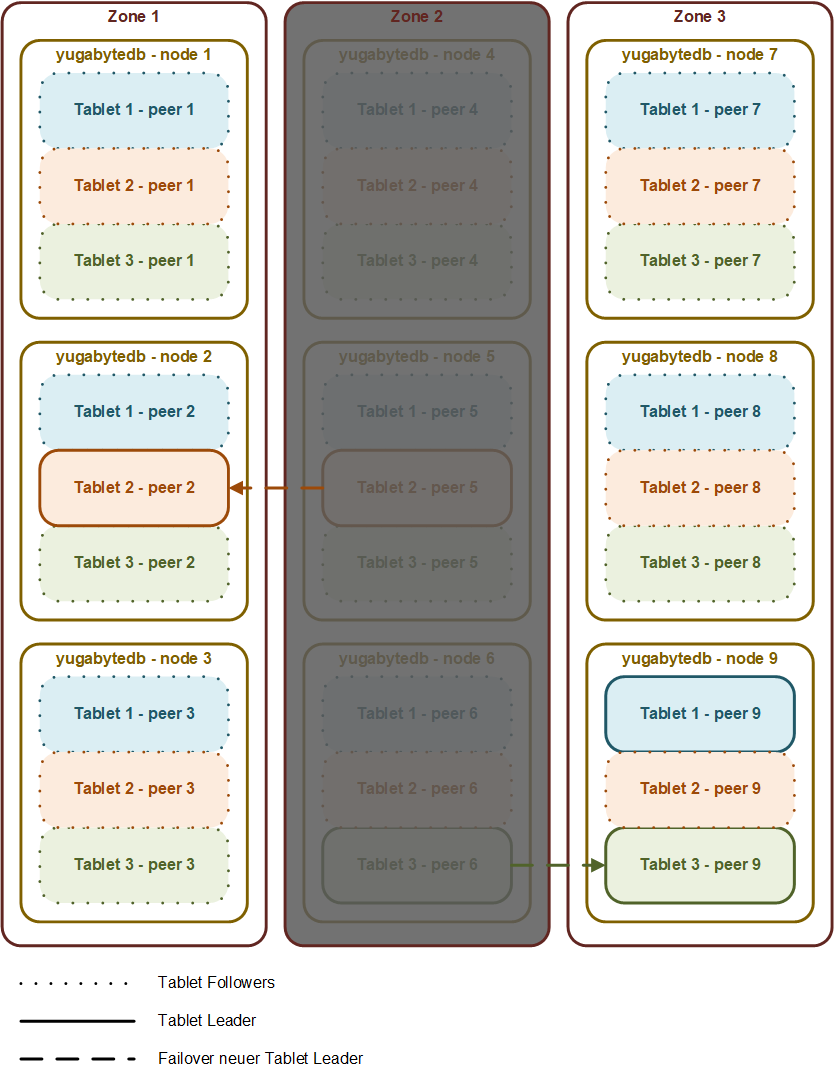
\includegraphics[width=0.8\linewidth]{source/implementation/evaluation/postgresql_ha_solutions/yugabytedb/yugabytedb-zone-outage-tolerance}
        \caption{yugabyteDB - Zone outage Tolerance}
        \label{fig:yugabytedb-zone-outage-tolerance}
    \end{figure}
\end{flushleft}
\begin{flushleft}
    \paragraph{Maintenance}
    \hyperref[subsec:maintenance_patroni]{Anhang - Maintenance}

\end{flushleft}
\begin{flushleft}
    \paragraph{Synergien und Mehrwert}
    Der grosse Benefit von YugabyteDB ist sein Distributed SQL Ansatz.
\end{flushleft}
\begin{flushleft}
    Zudem bietet YugabyteDB eine vollständige \Gls{Cassandra} Integration.\\
\end{flushleft}
\begin{flushleft}
    Der Benefit ist auf jeden Fall gegeben.
\end{flushleft}

